\documentclass{article}

\usepackage{fancyhdr} % Required for custom headers
\usepackage{lastpage} % Required to determine the last page for the footer
\usepackage{extramarks} % Required for headers and footers
\usepackage[usenames,dvipsnames]{color} % Required for custom colors
\usepackage{graphicx} % Required to insert images
\usepackage{listings} % Required for insertion of code
\usepackage{courier} % Required for the courier font
\usepackage{lipsum} % Used for inserting dummy 'Lorem ipsum' text into the template
\usepackage{amssymb}
\usepackage{tikz}

% Margins
\topmargin=-0.45in
\evensidemargin=0in
\oddsidemargin=0in
\textwidth=6.5in
\textheight=9.0in
\headsep=0.25in

\linespread{1.1} % Line spacing

% Set up the header and footer
\pagestyle{fancy}
\lhead{\hmwkAuthorName} % Top left header
\chead{\hmwkClass\ (\hmwkClassInstructor\ \hmwkClassTime): \hmwkTitle} % Top center head
\rhead{\firstxmark} % Top right header
\lfoot{\lastxmark} % Bottom left footer
\cfoot{} % Bottom center footer
\rfoot{Page\ \thepage\ of\ \protect\pageref{LastPage}} % Bottom right footer
\renewcommand\headrulewidth{0.4pt} % Size of the header rule
\renewcommand\footrulewidth{0.4pt} % Size of the footer rule

\setlength\parindent{0pt} % Removes all indentation from paragraphs

\definecolor{MyDarkGreen}{rgb}{0.0,0.4,0.0} % This is the color used for comments
\lstloadlanguages{Perl} % Load Perl syntax for listings, for a list of other languages supported see: ftp://ftp.tex.ac.uk/tex-archive/macros/latex/contrib/listings/listings.pdf
\lstset{language=Perl, % Use Perl in this example
        frame=single, % Single frame around code
        basicstyle=\small\ttfamily, % Use small true type font
        keywordstyle=[1]\color{Blue}\bf, % Perl functions bold and blue
        keywordstyle=[2]\color{Purple}, % Perl function arguments purple
        keywordstyle=[3]\color{Blue}\underbar, % Custom functions underlined and blue
        identifierstyle=, % Nothing special about identifiers
        commentstyle=\usefont{T1}{pcr}{m}{sl}\color{MyDarkGreen}\small, % Comments small dark green courier font
        stringstyle=\color{Purple}, % Strings are purple
        showstringspaces=false, % Don't put marks in string spaces
        tabsize=5, % 5 spaces per tab
        %
        % Put standard Perl functions not included in the default language here
        morekeywords={rand},
        %
        % Put Perl function parameters here
        morekeywords=[2]{on, off, interp},
        %
        % Put user defined functions here
        morekeywords=[3]{test},
       	%
        morecomment=[l][\color{Blue}]{...}, % Line continuation (...) like blue comment
        numbers=left, % Line numbers on left
        firstnumber=1, % Line numbers start with line 1
        numberstyle=\tiny\color{Blue}, % Line numbers are blue and small
        stepnumber=5 % Line numbers go in steps of 5
}

% Creates a new command to include a perl script, the first parameter is the filename of the script (without .pl), the second parameter is the caption
\newcommand{\perlscript}[2]{
\begin{itemize}
\item[]\lstinputlisting[caption=#2,label=#1]{#1.pl}
\end{itemize}
}

%----------------------------------------------------------------------------------------
%	DOCUMENT STRUCTURE COMMANDS
%	Skip this unless you know what you're doing
%----------------------------------------------------------------------------------------

% Header and footer for when a page split occurs within a problem environment
\newcommand{\enterProblemHeader}[1]{
\nobreak\extramarks{#1}{#1 continued on next page\ldots}\nobreak
\nobreak\extramarks{#1 (continued)}{#1 continued on next page\ldots}\nobreak
}

% Header and footer for when a page split occurs between problem environments
\newcommand{\exitProblemHeader}[1]{
\nobreak\extramarks{#1 (continued)}{#1 continued on next page\ldots}\nobreak
\nobreak\extramarks{#1}{}\nobreak
}

\setcounter{secnumdepth}{0} % Removes default section numbers
\newcounter{homeworkProblemCounter} % Creates a counter to keep track of the number of problems

\newcommand{\homeworkProblemName}{}
\newenvironment{homeworkProblem}[1][Problem \arabic{homeworkProblemCounter}]{ % Makes a new environment called homeworkProblem which takes 1 argument (custom name) but the default is "Problem #"
\stepcounter{homeworkProblemCounter} % Increase counter for number of problems
\renewcommand{\homeworkProblemName}{#1} % Assign \homeworkProblemName the name of the problem
\section{\homeworkProblemName} % Make a section in the document with the custom problem count
\enterProblemHeader{\homeworkProblemName} % Header and footer within the environment
}{
\exitProblemHeader{\homeworkProblemName} % Header and footer after the environment
}

\newcommand{\problemAnswer}[1]{ % Defines the problem answer command with the content as the only argument
    \noindent\framebox[\columnwidth][c]{
        \begin{minipage}{0.98\columnwidth}
            \textbf{Answer}

            #1
        \end{minipage}
    } % Makes the box around the problem answer and puts the content inside
}

\newcommand{\homeworkSectionName}{}
\newenvironment{homeworkSection}[1]{ % New environment for sections within homework problems, takes 1 argument - the name of the section
\renewcommand{\homeworkSectionName}{#1} % Assign \homeworkSectionName to the name of the section from the environment argument
\subsection{\homeworkSectionName} % Make a subsection with the custom name of the subsection
\enterProblemHeader{\homeworkProblemName\ [\homeworkSectionName]} % Header and footer within the environment
}{
\enterProblemHeader{\homeworkProblemName} % Header and footer after the environment
}

%----------------------------------------------------------------------------------------
%	NAME AND CLASS SECTION
%----------------------------------------------------------------------------------------

\newcommand{\hmwkTitle}{Assignment \#1} % Assignment title
\newcommand{\hmwkDueDate}{Thursday, September 5, 2013} % Due date
\newcommand{\hmwkClass}{CSCI 8950} % Course/class
\newcommand{\hmwkClassTime}{} % Class/lecture time
\newcommand{\hmwkClassInstructor}{Dr. Rasheed} % Teacher/lecturer
\newcommand{\hmwkAuthorName}{Yuchen Ying} % Your name

%----------------------------------------------------------------------------------------
%	TITLE PAGE
%----------------------------------------------------------------------------------------

\title{
\vspace{2in}
\textmd{\textbf{\hmwkClass:\ \hmwkTitle}}\\
\normalsize\vspace{0.1in}\small{Due\ on\ \hmwkDueDate}\\
\vspace{0.1in}\large{\textit{\hmwkClassInstructor\ \hmwkClassTime}}
\vspace{3in}
}

\author{\textbf{\hmwkAuthorName}}
\date{} % Insert date here if you want it to appear below your name

%----------------------------------------------------------------------------------------

\begin{document}

\maketitle

%----------------------------------------------------------------------------------------
%	TABLE OF CONTENTS
%----------------------------------------------------------------------------------------

%\setcounter{tocdepth}{1} % Uncomment this line if you don't want subsections listed in the ToC

\newpage
\tableofcontents
\newpage

%----------------------------------------------------------------------------------------
%	PROBLEM 1
%----------------------------------------------------------------------------------------

% To have just one problem per page, simply put a \clearpage after each problem

\begin{homeworkProblem}
    The goal of the Tic-Tac-Toe game is to place three X's or three O's on the same row, column or diagonal on a 3 by 3 board. If you never played it, or need more information about it, please visit \texttt{http://boulter.com/ttt/} or search for other sites on the web. Our objective in this problem is to learn a good strategy to play Tic-Tac-Toe.

    Formulate the Tic-Tac-Toe learning as a machine learning problem. You should briefly describe:

    \begin{itemize}
        \item What exactly would be learned and how it would be represented
        \item How the training examples will be obtained
        \item Which learning algorithm will be used
    \end{itemize}
    \problemAnswer{
        Tic-Tac-Toe learning problem:

        \begin{itemize}
            \item Task \texttt{T}: playing Tic-Tac-Toe
            \item Performance measure \texttt{P}: percent of games won against opponents
            \item Training experience \texttt{E}: playing practice games against itself
            \item Target function \texttt{V}: Board $\to$ $\mathbb{R}$
            \item Target function representation \texttt{\^{V}}: $\hat{V} = w_0 + w_1*{corner}_o + w_2*{corner}_x + w_3*{middle}_o + w_4*{middle}_x + w_5*{center}_o + w_6*{center}_x$

                where ${corner}_x$ means the count of \texttt{X}'s in one of the four corners, and ${middle}_x$ means the count of \texttt{X}'s in the middle of each side, and ${center}_x$ means the count of \texttt{X}'s in the center
        \end{itemize}

        \textbf{Knowledge to be learned}: for any given board status, choose the best move.

        \textbf{How this knowledge represented}: using an evaluation function that assign higher scores to better board stats.

        \textbf{How the training examples will be obtained}: human playing Tic-Tac-Toe.

        \textbf{Which learning algorithm will be used}: we can use the least mean squares (LMS) algorithm.
    }
\end{homeworkProblem}

\begin{homeworkProblem}
    Solve problem 2.4 on page 48 of the text book.

    Consider the instance space consisting of integer points in the $x$, $y$ plane and the set of hypotheses $H$ consisting of rectangles. More precisely, hypotheses are the form $a \le x \le b$, $c \le y \le d$, where $a$, $b$, $c$ and $d$ can be any integers.

    (a) Consider the version space with respect to the set of positive (+) and negative (-) training examples show below. What is the $S$ boundary of the version space in this case? Write out the hypotheses and draw them in on the diagram.

    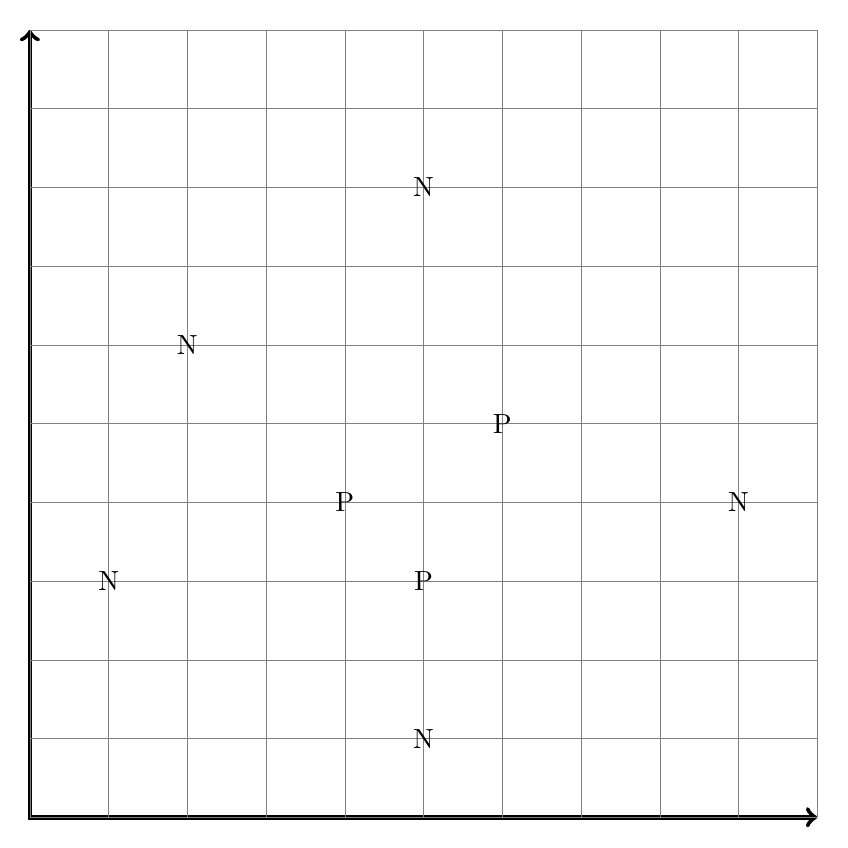
\begin{tikzpicture}
        \draw [ultra thick, <->] (0,10) -- (0,0) -- (10,0);
        \draw [help lines] (0,0) grid (10,10);
        \node (A) at (1,3) {N};
        \node (B) at (5,1) {N};
        \node (C) at (9,4) {N};
        \node (D) at (5,8) {N};
        \node (E) at (2,6) {N};
        \node (F) at (5,3) {P};
        \node (G) at (6,5) {P};
        \node (H) at (4,4) {P};
    \end{tikzpicture}

    \problemAnswer{
        $S = \{ <4, 6, 3, 5>\}$

        The red square below

        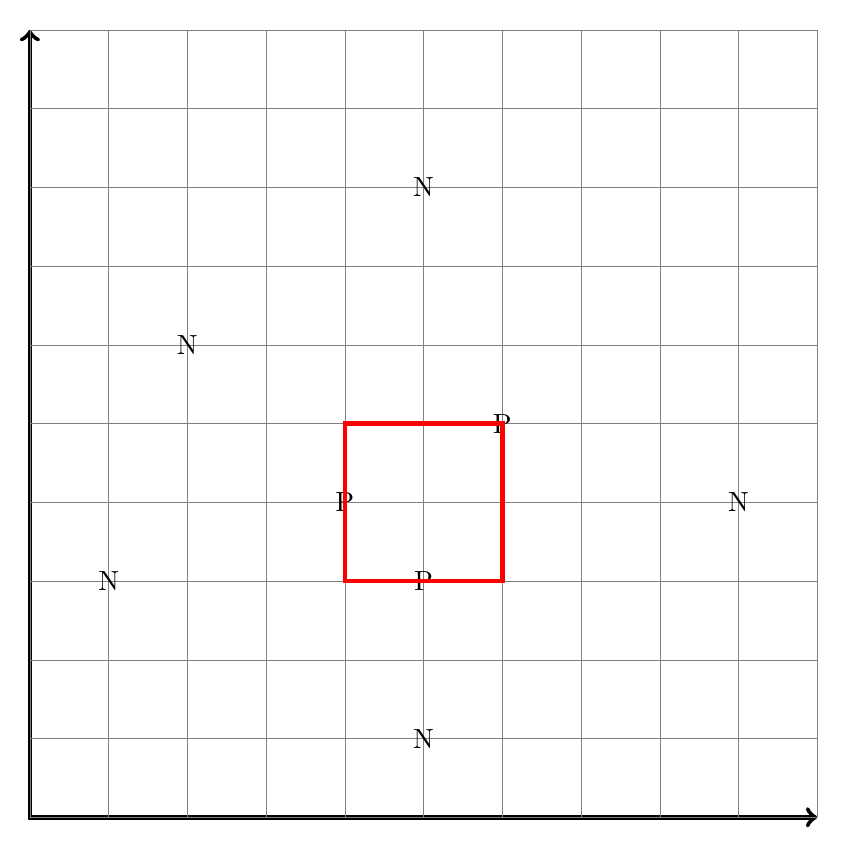
\begin{tikzpicture}
            \draw [ultra thick, <->] (0,10) -- (0,0) -- (10,0);
            \draw [help lines] (0,0) grid (10,10);
            \node (A) at (1,3) {N};
            \node (B) at (5,1) {N};
            \node (C) at (9,4) {N};
            \node (D) at (5,8) {N};
            \node (E) at (2,6) {N};
            \node (F) at (5,3) {P};
            \node (G) at (6,5) {P};
            \node (H) at (4,4) {P};
            \draw [ultra thick, red] (4,3) -- (4,5) -- (6,5) -- (6,3) -- cycle;
        \end{tikzpicture}
    }

    (b) What is the $G$ boundary of this version space? Write out the hypotheses and draw them in.

    \problemAnswer {
        $G = \{ <3, 8, 2, 7>, <2, 8, 2, 5>\}$

        The green and blue squares below

        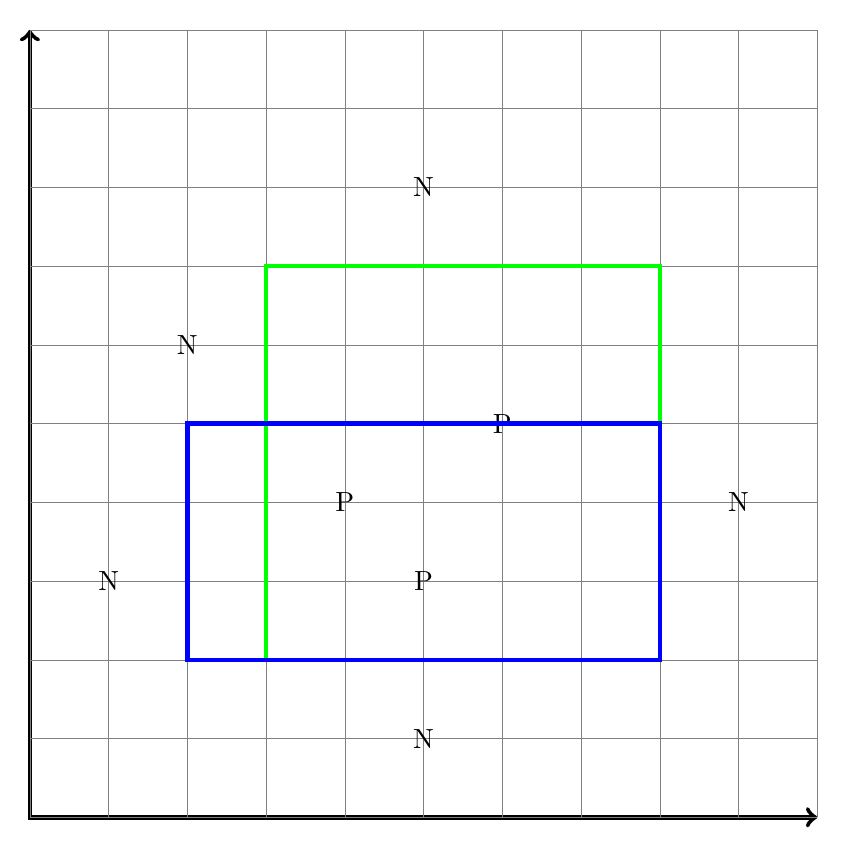
\begin{tikzpicture}
            \draw [ultra thick, <->] (0,10) -- (0,0) -- (10,0);
            \draw [help lines] (0,0) grid (10,10);
            \node (A) at (1,3) {N};
            \node (B) at (5,1) {N};
            \node (C) at (9,4) {N};
            \node (D) at (5,8) {N};
            \node (E) at (2,6) {N};
            \node (F) at (5,3) {P};
            \node (G) at (6,5) {P};
            \node (H) at (4,4) {P};
            \draw [ultra thick, green] (3,2) -- (8,2) -- (8,7) -- (3,7) -- cycle;
            \draw [ultra thick, blue] (2,2) -- (8,2) -- (8,5) -- (2,5) -- cycle;
        \end{tikzpicture}
    }

    (c) Suppose the learner may now suggest a new $x$, $y$ instance and ask the trainer for its classification. Suggest a query guaranteed to reduce the size of the version space, regardless of how the trainer classifies it. Suggest on that will not.

    \problemAnswer{
        Query that guaranteed to reduce the size of the version space: any point between $G$ and $S$, e.g. $(7,3)$

        Query that guaranteed not reduce the size of the version space: any point on the edge that belongs to both $G$ and $S$, e.g. $(5,5)$
    }

    (d) Now assume you are a teacher, attempting to teach a particular target concept (e.g. $3 \le x \le 5, 2 \le y \le 9$). What is the smallest number of training examples you can provide so that the \textsc{Candidate-Elimination} algorithm will berfectly learn the target concept?

    \problemAnswer{
        To learn $<3,5,2,9>$ perfectly, $S \equiv G$ when the training complete.

        $S$ needs to be described by two positive examples, and $G$ needs to be described by four negative examples.

        Positive examples: $<(3,9), (5,2)>$ or $<(3,2), (5,9)>$

        Negative examples (many possibilities): $<(2, 8), (4,10), (4,1), (6,3)>$
    }
\end{homeworkProblem}

\begin{homeworkProblem}
    Consider the \texttt{EnjoySport} concept learning task defined in Table 2.2 of the textbook.

    (a) Give a minimum length sequence of training examples that produces the following version space (represented by its \texttt{S} and \texttt{G} sets):

    \[
        \begin{array}{ccccccc}
            S:\{< & ? & \texttt{Warm} & \texttt{Normal} & \texttt{Strong} & \texttt{Cool} & ? >\} \\
            G:\{< & ? & ? & ? & ? & ? & ? >\}
        \end{array}
    \]

    \problemAnswer{
        \[
            \begin{array}{ccccccc}
                POSITIVE: < & \texttt{Sunny} & \texttt{Warm} & \texttt{Normal} & \texttt{Strong} & \texttt{Cool} & \texttt{Same} > \\
                POSITIVE: < & \texttt{Rainy} & \texttt{Warm} & \texttt{Normal} & \texttt{Strong} & \texttt{Cool} & \texttt{Change} > \\
                POSITIVE: < & \texttt{Cloudy} & \texttt{Warm} & \texttt{Normal} & \texttt{Strong} & \texttt{Cool} & \texttt{Change} > \\
            \end{array}
        \]
    }

    (b) Given a minimum length sequence of \textbf{additional} training examples that will transform the version space described above into the following version space:

    \[
        \begin{array}{ccccccc}
            S:\{< & ? & \texttt{Warm} & \texttt{Normal} & \texttt{Strong} & \texttt{Cool} & ? >\} \\
            G:\{< & ? & ? & \texttt{Normal} & \texttt{Strong} & ? & ? >\}
        \end{array}
    \]

    \problemAnswer{
        \[
            \begin{array}{ccccccc}
                NEGATIVE: < & \texttt{Sunny} & \texttt{Warm} & \texttt{High} & \texttt{Strong} & \texttt{Cool} & \texttt{Same} > \\
                NEGATIVE: < & \texttt{Sunny} & \texttt{Warm} & \texttt{Normal} & \texttt{Weak} & \texttt{Cool} & \texttt{Same} > \\
                NEGATIVE: < & \texttt{Sunny} & \texttt{Warm} & \texttt{High} & \texttt{Weak} & \texttt{Cool} & \texttt{Same} > \\
            \end{array}
        \]
    }
\end{homeworkProblem}

\begin{homeworkProblem}
    Consider the following examples for machine learning:

    \[
        \begin{tabular}{|c|c|c|c|c|c|c|}
            \hline
            Example & a1 & a2 & a3 & a4 & a5 & label \\
            \hline
            1 & 1 & 0 & 0 & 0 & 1 & + \\
            \hline
            2 & 1 & 1 & 1 & 0 & 0 & + \\
            \hline
            3 & 0 & 0 & 0 & 1 & 1 & - \\
            \hline
            4 & 1 & 0 & 1 & 0 & 0 & + \\
            \hline
        \end{tabular}
    \]

    Each hypothesis is described by a conjunction of constraints on the attributes \textbf{a1} through \textbf{a5}. The constraints may be ``*'' (any value is acceptable), ``$\emptyset$'' (no value is acceptable), or a specific value (i.e. 0 or 1)

    (a) Give the sequence of \texttt{S} and \texttt{G} boundary sets computed by the \textbf{Candidate-Elimination} algorithm going through the given examples in the given order.

    \problemAnswer{
        \[
            \begin{array}{rcccc}
                S_0 = \{(\emptyset,& \emptyset,& \emptyset,& \emptyset,& \emptyset)\} \\
                G_0 = \{(*,& * ,& * ,& * ,& *)\} \\
                \\
                S_1 = \{(1,& 0,& 0,& 0,& 1)\} \\
                G_1 = \{(*,& * ,& * ,& * ,& *)\} \\
                \\
                S_2 = \{(1,& *,& *,& 0,& *)\} \\
                G_2 = \{(*,& * ,& * ,& * ,& *)\} \\
                \\
                S_3 = \{(1,& *,& * ,& 0,& *)\} \\
                G_3 = \{(1,& *,& * ,& * ,& *), \\
                        (*,& *,& * ,& 0 ,& *)\} \\
                \\
                S_4 = \{(1,& *,& * ,& 0,& *)\} \\
                G_4 = \{(1,& *,& * ,& * ,& *), \\
                        (*,& *,& * ,& 0 ,& *)\} \\
            \end{array}
        \]
    }

    (b) Would the final version space obtained above change if the examples were considered in reverse order? Briefly explain why.

    \problemAnswer{
        Version space obtained won't change.

        If the version space changed (shrink or grow), that means learning the same example has different information gain, which is impossible.
    }

    (c) Give a minimum length sequence of \textbf{additional} training examples that will make the version space converge to one and only one hypothesis.

    \problemAnswer{
        The easiest way to do this is to make hypothesis in $G$ more specify. We need to find negative examples that makes the hypothesis in $G$ too general.

        $Negative: (1, *, *, 1, *)$: The first hypothesis in $G$ is not consist with this example, thus it needs to be more specify. So we remove it and add back $(1, *, *, 0, *)$

        $Negative: (0, *, *, 0, *)$: The second hypothesis in $G$ is not consist with this example, thus it needs to be more specify. So we remove it and add back $(1, *, *, 0, *)$

        In the end we get $S = \{(1, *, *, 0, *)\}$ and $G = \{(1, *, *, 0, *)\}$, this version space contains only one hypothesis.
    }
\end{homeworkProblem}
\end{document}
